\chapter{Implementatie}

	\par In dit hoofdstuk zal de implementatie van het volledige systeem besproken worden. Er zal vooral de nadruk gelegd worden op de moeilijkheden en problemen die zich voordeden tijdens het ontwikkelproces.

	\section{PID regelaar}

		\par De PID regelaar vormt het belangrijkste onderdeel van de quadcoptersturing. Deze component zal per as ge\"implementeerd moeten worden. Daarnaast kan de PID in een verder stadia ook gebruikt worden om de hoogte te stabiliseren. Er dient dus een flexibele component ontworpen te worden die meerdere malen ingezet kan worden. Hierbij is het belangrijk dat de waarden voor K\textsubscript{p}, K\textsubscript{i} en K\textsubscript{d} per controller ingesteld kunnen worden. Daarnaast is het ook mooi meegenomen om deze real-time aanpasbaar te maken. 

		\par De PID controller werd ontwikkeld in drie iteraties. Vanwege de hardware beperkingen van de FPGA was het nodig om een volledig re-design uit te voeren van de component. Deze stappen zullen hieronder verder toegelicht worden.

		\subsection{PID controller door middel van DSP48A slices}

			\par Vanuit theoretisch oogpunt zijn DSP48 slices ideaal voor het implementeren van een PID regelaar. De bewerkingen die uitgevoerd dienen te worden beperken zich tot optellen en vermenigvuldigen (MAC). Op deze manier wordt een hoge snelheid van de component mogelijk. Per PID regelaar zijn vier DSP48 slices nodig. In figuur \ref{pid_dsp48} is de onderverdeling weergegeven van DSP48 slices binnen de PID regelaar. Hierbij zijn de functies van slice 2 en 3 exact hetzelfde. Bij de laatste DSP48 slice is een terugkoppeling voorzien. Om ervoor te zorgen dat het resultaat nooit overflowt, dient er een downscaling te gebeuren bij de terugkoppeling. Deze wordt in \textquotesingle gewone\textquotesingle   logica uitgevoerd en zal het proces vertragen. Door het introduceren van de nodige \textquotesingle pipes\textquotesingle  wordt de maximale snelheid van implementatie bereikt.
				
				\begin{figure}[H]					  
					  \centering
					  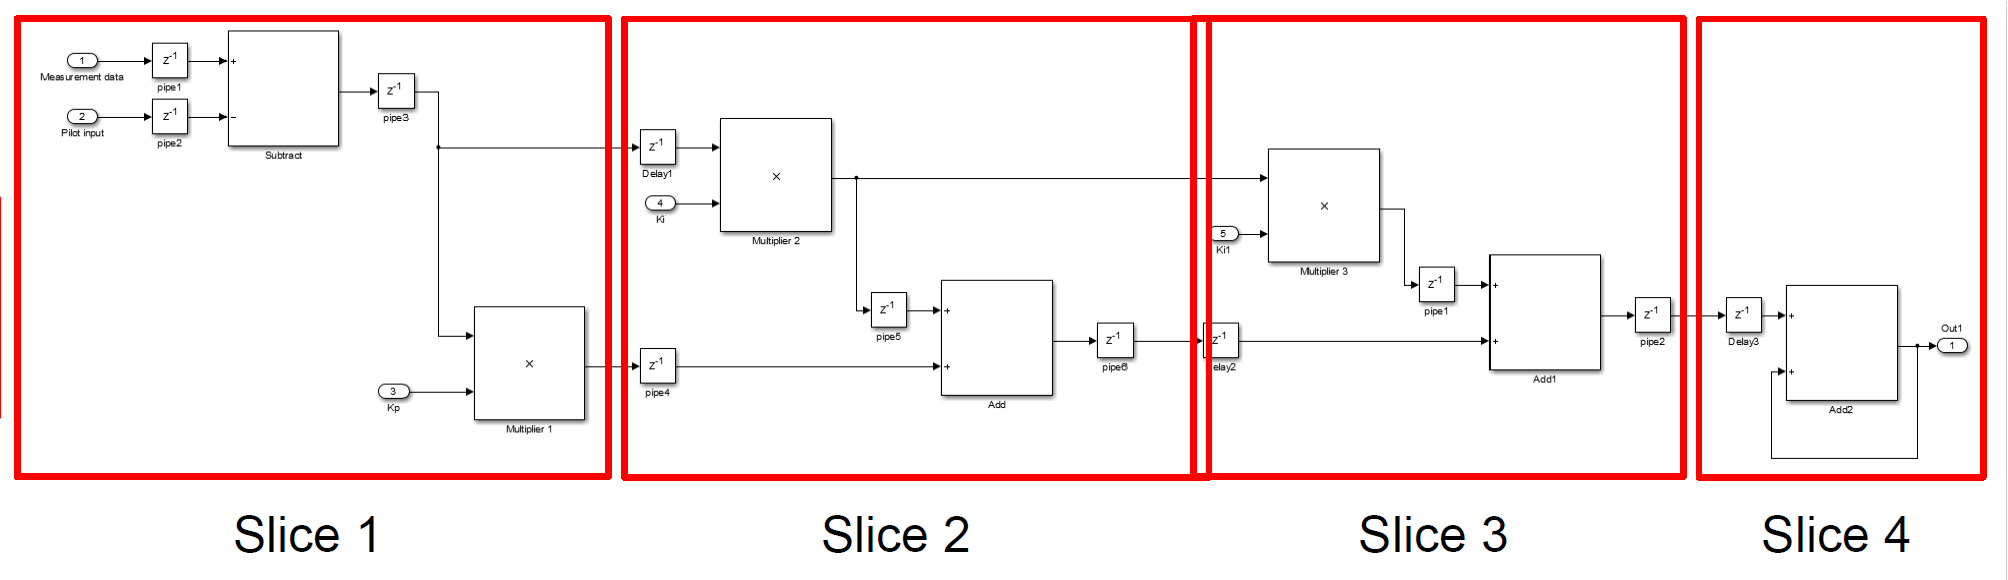
\includegraphics[width=\textwidth]{Implementatie/pid_dsp48.png}
					  \caption{Overzicht van een PID controller op basis van DSP48 slices}
					  \label{pid_dsp48}
				\end{figure}

			\par Bovenstaande code werd in een eerste fase ge\"implementeerd door middel van de Xilinx System Generator. Wanneer de VHDL code gegenereerd diende te worden, doken er steeds fouten op. Opzoekwerk heeft uitgewezen dat de System Generator niet compatibel is met Windows 8. Een Windows 7 apparaat met alle nodige software en licenties was helaas niet beschikbaar. Er werd overgegaan naar het implementeren van de PID in Xilinx ISE. Hierbij werd gebruik gemaakt van de IP Coregen voor het genereren van de juiste instellingen binnen de DSP48 slices.

			\par Door eerste synthese resultaten bleek dat het niet mogelijk was om drie of vier PID's te implementeren op de Spartan 6 FPGA wegens gebrek aan resources. Een mogelijke oplossing was het multiplexen van de PID regeling. Op die manier is er slechts \'e\'en PID regelaar nodig die afwisselend de berekeningen uitvoert voor een bepaald kanaal. De implementatie hiervan bleek echter te complex om te realiseren omdat de PID steeds de vorige resultaten nodig heeft om het volgende te berekenen. Deze data zou dus moeten opgeslagen worden. Daarnaast was het ook niet steeds mogelijk om deze waarden terug op de juiste plaats in het DSP48 slice te laden vanwege de beperkingen van ingangssignalen.

			\par Er dient dus een andere oplossing gevonden te worden om de PID in de Spartan 6 FPGA te implementeren.

		\subsection{PID controller door middel van IPCore multiplier}
		\label{pid_mult}

			\par Een tweede aanpak was om de PID te implementeren aan de hand van \textquotesingle gewone\textquotesingle  logica. Om de vermenigvuldigingen uit te voeren wordt gebruik gemaakt van de IP Core multiplier. Er zijn dus drie van deze multipliers nodig om de volledige component te realiseren. 

			\par Bij het aanmaken van deze multipliers zijn verschillende keuzes mogelijk. Er kan gekozen worden tussen een implementatie die gebruik maakt van ExtremeDSP (DSP48A slices) of een implementatie die gebruik maakt van LUT's en FF. Afhankelijk van de gekozen optie zullen de timings verschillen. Er is ook een mogelijk om te optimaliseren naar area (minimaal gebruik aan resources) of naar snelheid. Er werd gekozen om te minimaliseren naar area. Hierbij maakte de multiplier enkel gebruik van LUT's en FF. 

			\par Via Xilinx Vivado werd een eerste versie van deze PID ge\"implementeerd en gesimuleerd. De keuze voor Vivado werd gemaakt omwille van problemen met de ISE simulator op Windows 8. Daarnaast was het ook niet mogelijk om CoreIP componenten te simuleren in Modelsim vanwege een probleem met de bibliotheken. Xilinx biedt deze niet meer aan, omdat zij een eigen simulator ontwikkeld hebben.

			\par De simulaties leverden dezelfde resultaten op als bekomen in Simulink. Er kon dus besloten worden dat de implementatie van de PID gelijkaardig is als de versie in Simulink. Bij het verder onderzoeken van de synthese resultaten bleek dat er op het eerste zicht voldoende resources beschikbaar waren om vier PID controllers te implementeren. Omdat er niet enkel een PID op de FPGA ge\"implementeerd moet worden, maar ook nog een reeks andere componenten zou het toch kunnen dat men niet voldoende resources ter beschikking heeft.

			\par  Er dient dus een andere oplossing gevonden te worden om de PID in de Spartan 6 FPGA te implementeren met een minimaal gebruik aan resources.

		\subsection{PID controller door middel van multiplexed IPCore multiplier}			

			\par Een oplossing om de resources binnen een PID controller aanzienlijk te beperken is door in plaats van drie multipliers slechts \'e\'en multiplier te gebruiken. Hierbij zal telkens de P, I en D actie uitgevoerd worden. De snelheid van het component zal hierdoor dalen met ongeveer een facor drie, maar dit zal weinig invloed hebben op de werking van de autopilot. Aangezien de sensordata binnenkomt met een snelheid van enkele kHz en de PID component geklokt kan worden aan een snelheid van enkele MHz zal hier geen effect van opgemerkt kunnen worden.

			\par De implementatie gebeurt door middel van een state machine. In een eerste state zullen de  K\textsubscript{p}, K\textsubscript{i} en K\textsubscript{d} waarden ingelezen worden. Op deze manier zijn ze per berekening real-time aanpasbaar. In de volgende states zullen de P, I en D acties uitgevoerd worden. Dit houdt in dat de data die aan de multiplier aangelegd wordt, wijzigt per state. In de laatste state wordt een vlag kort hoog geplaatst om aan te geven dat de berekening klaar is. Er is dus maar \'e\'en multiplier nodig die gemultiplext wordt.

			\par Door het beperken van het aantal multipliers kon de snelheid van de multiplier geoptimaliseerd worden door toch gebruik te maken van DSP48 slices binnen deze multiplier. Deze wijziging werd dan ook doorgevoerd in de component.
\newpage
			\par Simulaties van de bovenstaande PID leverden exact hetzelfde resultaat op als de PID beschreven in paragraaf \ref{pid_mult}. Een overzicht van deze testbench is weergegeven in figuur \ref{pid_tb_mult}.

				\begin{figure}[H]					  
					  \centering
					  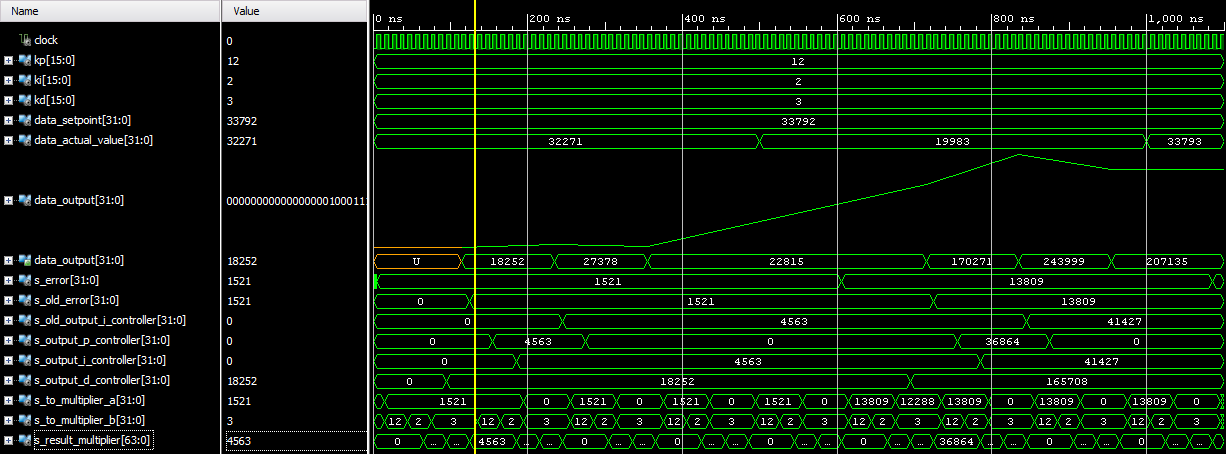
\includegraphics[width=\textwidth]{Implementatie/pid testbench.png}
					  \caption{Simulatieresultaat van PID regelaar met gemultiplext multiplier}
					  \label{pid_tb_mult}
				\end{figure}

			\par Wanneer men figuur \ref{pid_tb_mult} nader bekijkt, kan men opmerken dat wanneer de wenswaarde bereikt is, en bijgevolg het errorsignaal 0 is, de uitvoer niet terugvalt naar 0. De reden hiervoor is eenvoudig te verklaren. Aangezien de testbench werkt door middel van het aanleggen van bepaalde signalen voor gemeten waarde op bepaalde tijdstippen, heeft men hier niet te maken met een echt systeem. De I actie van de PID wordt berekend door middel van volgende formule.

				\[ I\textsubscript{regelaar} = (Error \cdot K\textsubscript{i} + Old_K\textsubscript{i} ) \] 

			\par Er wordt dus steeds een berekening gemaakt op basis van de oude waarde van K\textsubscript{i} waardoor de waarde nooit 0 wordt in de simulatie. In een echt systeem wordt dit probleem onmiddellijk opgelost omdat de regelaar zal blijven bijregelen. De sensor zal opmerken dat de waarde de wens overstijgt en een tegenactie ondernemen. 


		\subsection{Samenvattig PID controller}

			\par In listing \ref{PID_list_1} is de componentdefinitie van de PID controller weergegeven. Als invoer zijn zowel de sensordata als de gewenste waarde nodig. Daarnaast moeten ook de co\"effici\"enten voor  K\textsubscript{p}, K\textsubscript{i} en K\textsubscript{d} aangelegd worden. Deze co\"effici\"enten zijn real-time aanpasbaar.
\newpage
			\par Door de PID regelaar in verschillende stappen te ontwerpen konden steeds resources bespaard worden. Dit ging wel steeds ten koste van de snelheid van de component. Hoge snelheid bij deze component is niet zo belangrijk vanwege de relatief trage snelheid weermee de invoerdata kan aangeleverd worden. 

				\lstinputlisting[style=vhdl, caption=Overzicht van de PID component, label=PID_list_1]{Implementatie/pid.vhd}

	\section{PWM generator}

		\par Per motor is er telkens \'e\'en PWM generator nodig bij de quadcopter. De PWM generator zal een PWM signaal genereren op basis van een invoerwaarde die afkomstig is van de motormixing component. Om flexibiliteit te garanderen is de component volledig generiek gemaakt. Op deze manier kan zowel de resolutie als PWM frequentie gewijzigd worden. Een overzicht van de PWM component is weergegeven in listing \ref{pwm_gen}. 

			\lstinputlisting[style=vhdl, caption=Overzicht van de PWM component, label=pwm_gen]{Implementatie/pwm_gen.vhd}

	\section{Motor Mixing}

		\par Het motormixing gedeelte van de quadcopter is verantwoordelijk voor het genereren van de signalen die naar elke motor gestuurd moeten worden. Bij de opbouw van de quadcopter werd gekozen voor de \textquotesingle +\textquotesingle  configuraties. Het mixen van de motors gebeurt dan via het volgend algoritme.

			\[ Motor\textsubscript{front} = baseSnelheid + pitchOutput - yawOutput \]
			\[ Motor\textsubscript{left} = baseSnelheid + rollOutput + yawOutput \]
			\[ Motor\textsubscript{back} = baseSnelheid - pitchOutput - yawOutput \]
			\[ Motor\textsubscript{right} = baseSnelheid - rollOutput + yawOutput \]

		\par Hierbij is de baseSnelheid gelijk aan de idle snelheid van de motor vermeerderd met de throttle.

		\par Net als bij de PWM generator is ook deze component volledig generiek opgebouwd zodat deze makkelijk kan aangepast worden. Een overzicht van deze component is weergegeven in listing \ref{motormixing}.

			\lstinputlisting[style=vhdl, caption=Overzicht van de motormixing component, label=motormixing]{Implementatie/motormixing.vhd}

		\par Er zal ook rekening gehouden worden met de maxima waarde van het systeem. Wanneer een bepaalde waarde het maximum overschrijdt zal deze waarde automatisch worden teruggebracht naar de maximum waarde. De corrigerende actie zal daarom wat minder zijn dan gevraagd, maar de quadcopter blijft op deze manier wel binnen zijn limieten.

	\section{SPI slave interface}

		\par Zoals reeds eerder vermeld werd, voorziet de SPI interface de mogelijkheid om de autopilot te laten communiceren met de buitenwereld. In het vooronderzoek werd reeds de werking van een SPI slave interface aangehaald. Deze is in VHDL ge\"implementeerd voor CPOL en CPHA waarbij beiden gelijk zijn aan 0. Als databreedte werd gekozen voor 8 bits, ofwel 1 byte.

		%\par Via de SPI slave interface is het ook mogelijk om toegang te krijgen tot de analoge pinnen van het Mojo board. Dit kan in het verdere verloop van het project nodig zijn. 

		\par In  listing \ref{spi_slave} is een overzicht weergegeven van het SPI slave component. Er kan data ingevoerd worden die verstuurd moet worden. Daarnaast wordt er ook kort een vlag hoog geplaatst wanneer de data ontvangen is.

			\lstinputlisting[style=vhdl, caption=Overzicht van de SPI slave component, label=spi_slave]{Implementatie/spi_slave.vhd}

		\par Om de werking van deze component te valideren, is er een testbench voor deze component ontworpen. Deze wordt geanalyseerd alvorens de code te testen op het Mojo board. Het resultaat van deze testbench is weergegeven in figuur \ref{spi_slave_tb}.

				\begin{figure}[H]					  
					  \centering
					  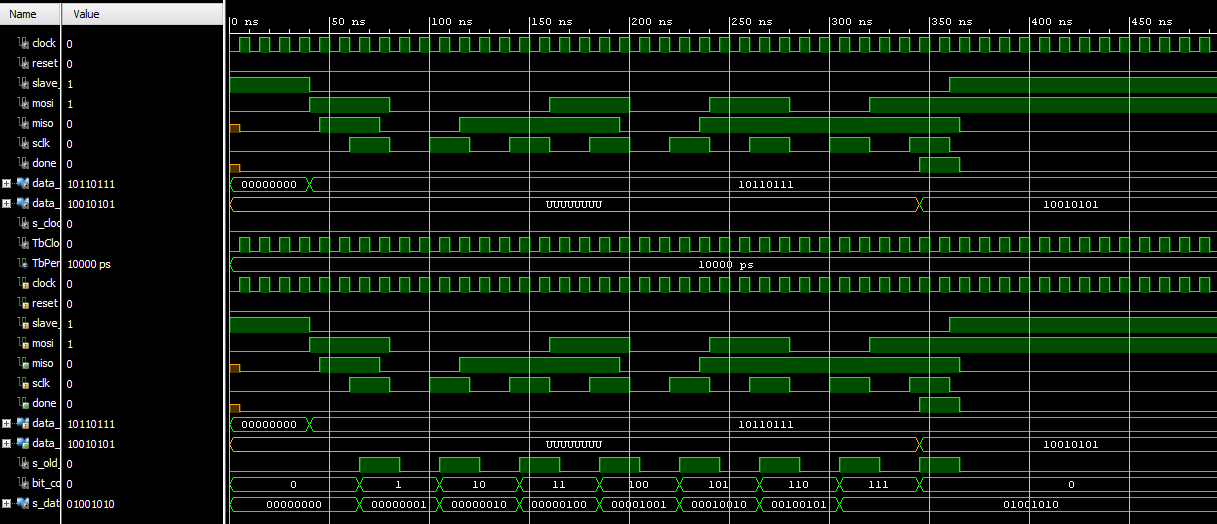
\includegraphics[width=0.9\textwidth]{Implementatie/spi_tb.png}
					  \caption{Simulatieresultaat van SPI slave interface}
					  \label{spi_slave_tb}
				\end{figure}

	\section{Top level}

		\par Het toplevel verbindt alle systeemcomponenten met elkaar. Daarnaast is ook op dit niveau de register ge\"implementeerd aan de hand van de IP Coregen. Er wordt gebruik gemaakt van een block memory met 255 registers die elk een grootte hebben van 1 byte. Via de SPI interface kunnen deze registers zowel gelezen als ingesteld worden.

		\par Het toplevel zal ook de nodige signalen naar de buitenwereld brengen. Zo worden de signalen naar de motoren, SPI-apparaten en sensoren naar buiten gebracht. 

		\par Via de IP Core clocking wizard worden de verschillende klokken aangemaakt waarmee de componenten werken. 

	\section{Quadcopter Frame}

		\par Niet alleen de hardware componenten werden ontwikkeld tijdens dit projectlab, ook de quadcopter zelf werd ontworpen. Hierbij wordt gebruik gemaakt van een 3D printer die de verschillende onderdelen zal vervaardigen. In het computerprogramma Inventor worden alle onderdelen getekend en klaargemaakt om te kunnen worden geprint.

		\par Een quadcopter is opgebouwd uit vier armen die gepositioneerd zijn in een \textquotesingle x\textquotesingle. Zo\textquotesingle n arm is weergegeven in figuur \ref{quad_frame_pict}. 

			\begin{figure}[H]					  
				  \centering
				  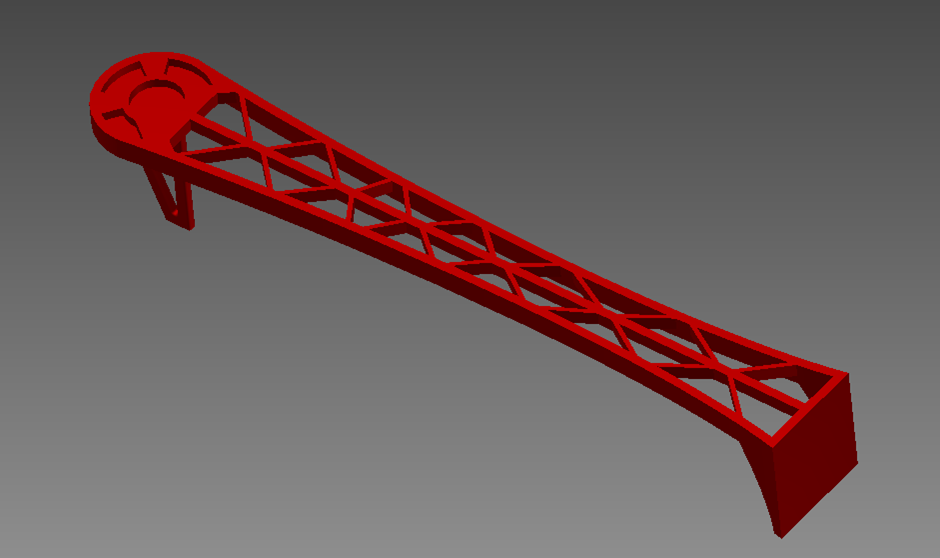
\includegraphics[width=0.6\textwidth]{Implementatie/frame.png}
				  \caption{Weergave van een quadcopter arm}
				  \label{quad_frame_pict}
			\end{figure}

		\par De frameonderdelen werden vervaardigd door middel van een Ultimaker 3D printer. Indien er tijdens de vlucht een bepaald onderdeel beschadigd raakt, kan dit makkelijk opnieuw geprint worden en is quadcopter snel weer operatief. Het printen van een arm neemt ongeveer 4 uur in beslag.





